\section{Results}

\frame
{
	\frametitle{Results}

	\begin{itemize}
	  \item \textbf{Objective}: Evaluate evolution of mimicry.
	  \item \textbf{Evaluation process}:
			\begin{itemize}
			  \item Calculate number mimicry rings.
			  \item Calculate size of mimicry rings:
					\begin{itemize}
					  \item Population of \textit{palatable} species.
					  \item Population of \textit{unpalatable} species.
					\end{itemize}			  
			\end{itemize}
		\item \textbf{Report parameters}:
			\begin{table}
			\centering
			\begin{scriptsize}
			\begin{spacing}{1.5}
			\begin{tabular}{| l | c |}
				\hline
					\textbf{Parameter} & \textbf{Value} \\ \hline
					Mimicry Ring hamming distance & 10 \% of the Pattern Size \\ \hline
					Number of Rings to report & 8 \\
				\hline
			\end{tabular}
			\end{spacing}
			\end{scriptsize}
			\caption{Parameters to mimicry ring report.}
			\label{tab:ring-report-control-parameters}
			\end{table}		
	\end{itemize}
}

\subsection{Experiments}

%-----------------------------
%----- Two Prey Species ------
%-----------------------------

\frame
{
	\frametitle{Two Prey Species}
	\framesubtitle{Initial Configuration}

	\begin{table}
	\centering
	\begin{tiny}
	\begin{spacing}{1.5}
	\begin{tabular}{|l|l|c|c|l|c|}
	  \hline
	   														&\multicolumn{3}{c|}{Prey configuration} 																	
	   														& \multicolumn{2}{c|}{Predator configuration} \\ \hline
	  \multirow{2}{*}{Population} & Rule110 (Palatable) & \parbox[c]{2.1em}{
\includegraphics[scale=0.30]{../tex/images/CARule110}} & 108 
	  														& \multicolumn{2}{c|}{\multirow{2}{*}{10}} \\ \cline{2-4}
	  					 									& Rule30 (Unpalatable)& \parbox[c]{2.1em}{
\includegraphics[scale=0.30]{../tex/images/CARule30}}  & 108 
	  					 									& \multicolumn{2}{c|}{}\\ \hline
	  \multirow{2}{*}{Reproduction} & Age Limit & \multicolumn{2}{c|}{100}  & \multicolumn{2}{c|}{500} \\ \cline{2-6}
	  						 									& Interval  & \multicolumn{2}{c|}{1000} & \multicolumn{2}{c|}{1200} \\ \hline
	  \multirow{2}{*}{Mutation Rate} & Pattern   & \multicolumn{2}{c|}{0.05}& \multicolumn{2}{c|}{\multirow{2}{*}{0.3}} \\ \cline{2-4}
	  						 									 & Genome    & \multicolumn{2}{c|}{0.5} & \multicolumn{2}{c|}{} \\ \hline
	  Demise Age	 									 & \multicolumn{3}{c|}{2000}						& \multicolumn{2}{c|}{2500} \\ \hline
	  Minimum Attack Age						 & \multicolumn{3}{c|}{} 						    & \multicolumn{2}{c|}{500} \\ \hline
	  \multirow{2}{*}{Memory Configuration} & \multicolumn{3}{c|}{} 					& Minimum & 2 \\ \cline{5-6}
	   																			& \multicolumn{3}{c|}{} 					& Maximum & 10 \\ \hline  
	\end{tabular}
	\end{spacing}
	\end{tiny}
	\caption{Agent configuration of 2 prey species}
	\label{tab:config-table-2-prey}
	\end{table}
}

\frame
{
	\frametitle{Two Prey Species}
	\framesubtitle{Population vs. Time (10k)}
	
	\begin{figure}
		\centering
		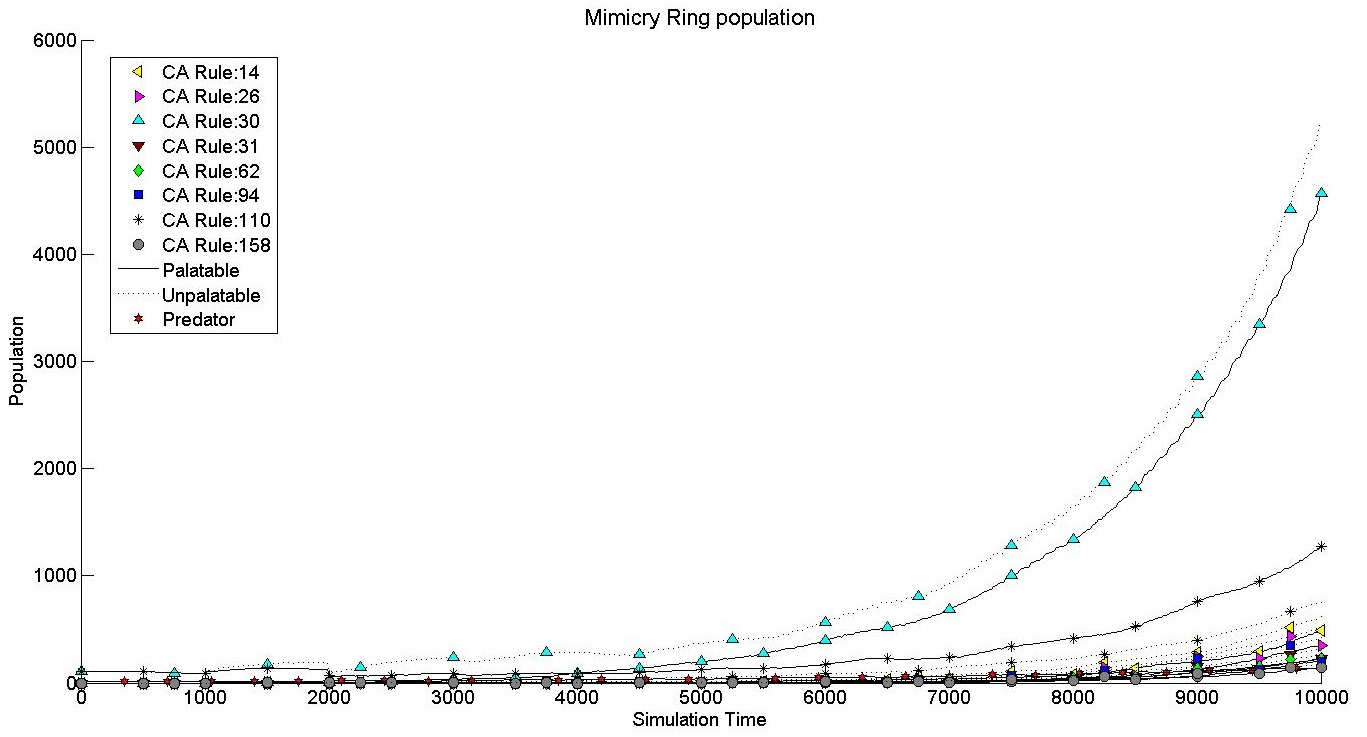
\includegraphics[scale=0.25]{../tex/images/simTime10k-2Prey}
		\caption{Population distribution of mimicry rings, initialized with 2 prey species, 10k iterations}
		\label{fig:plot-2-prey}
	\end{figure}
}

\frame
{
	\frametitle{Two Prey Species}
	\framesubtitle{Population vs. Time (5k)}
	
	\begin{figure}
		\centering
		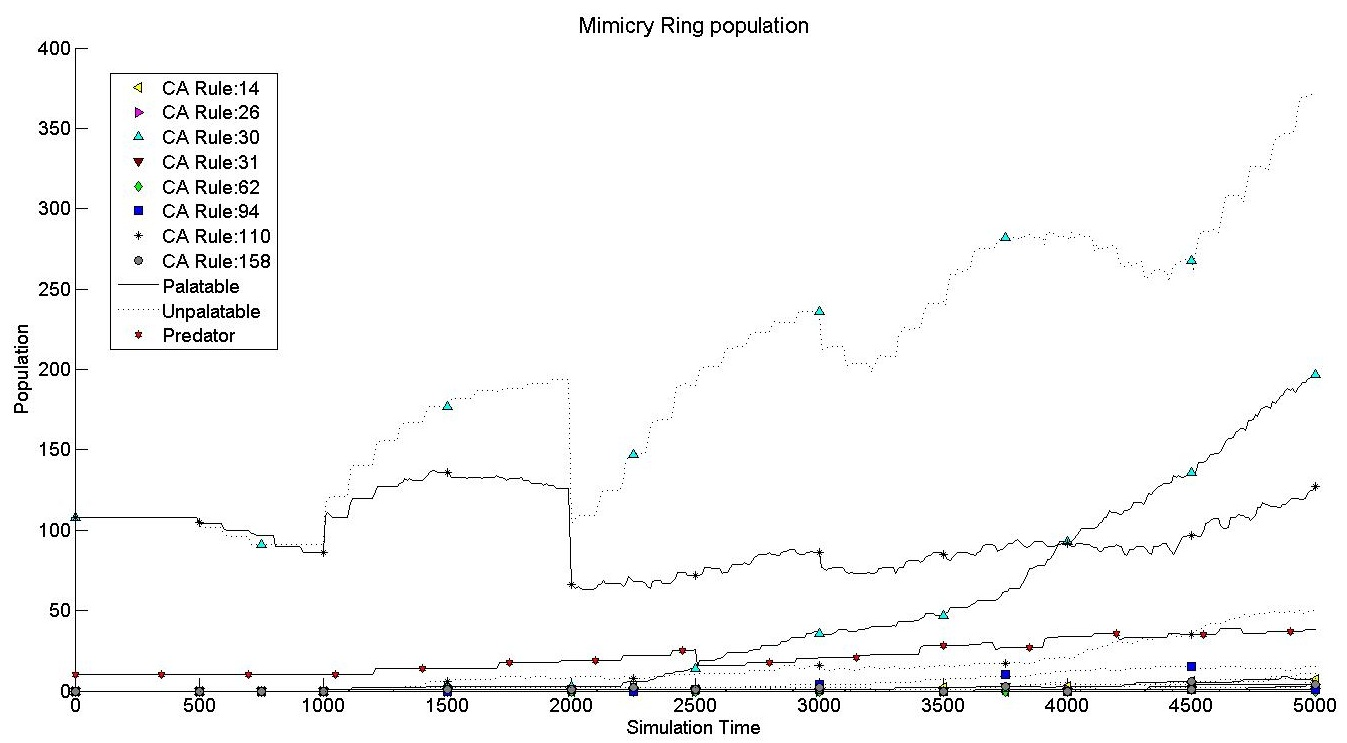
\includegraphics[scale=0.25]{../tex/images/simTime5k-2Prey}
		\caption{Population distribution of mimicry rings (2 prey species, 5k iterations)}
		\label{fig:plot-2-prey-5k}
	\end{figure}
}

\frame
{
	\frametitle{Two Prey Species}
	\framesubtitle{Number of Mimicry Rings}

	\begin{figure}[H]
		\centering
		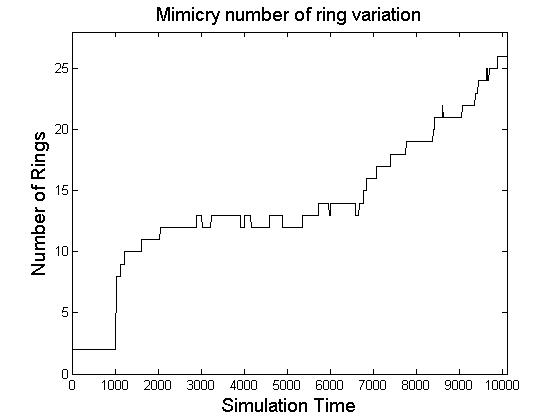
\includegraphics[scale=0.30]{../tex/images/ringSize10k-2Prey}
		\caption{Number of mimicry rings, initialized with 2 prey species.}
		\label{fig:ringSize10k-2Prey}
	\end{figure}	
}

\frame
{
	\frametitle{Prey Pattern}
	\framesubtitle{Genotype vs. Phenotype}
	
	\begin{itemize}
		\item Genetic bit difference of one.
		\item Vastly different phenotype.
	\end{itemize}
	
	\begin{table}
	\centering
	\begin{scriptsize}
	\begin{tabular}{|l|c|c|c|}
	  \hline
	  CA Rule & \(60 \equiv 00111100\) & \(61 \equiv 00111101\) & \(62 \equiv 00111110 \) \\ \hline
	  Pattern & \parbox[c]{2.1em}{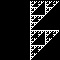
\includegraphics[scale=0.40]{../tex/images/CARule60}} 
	  				& \parbox[c]{2.1em}{
\includegraphics[scale=0.40]{../tex/images/CARule61}} 
	  				& \parbox[c]{2.1em}{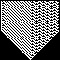
\includegraphics[scale=0.40]{../tex/images/CARule62}}\\
	  \hline
	\end{tabular}
	\end{scriptsize}
	\caption{Difference in prey pattern genotype and phenotype}
	\label{tab:diff-in-pattern}
	\end{table}
}

\frame
{
	\frametitle{Generated Prey Species}
	\framesubtitle{Population vs. Time (10k)}
	
	\begin{figure}[H]
		\centering
		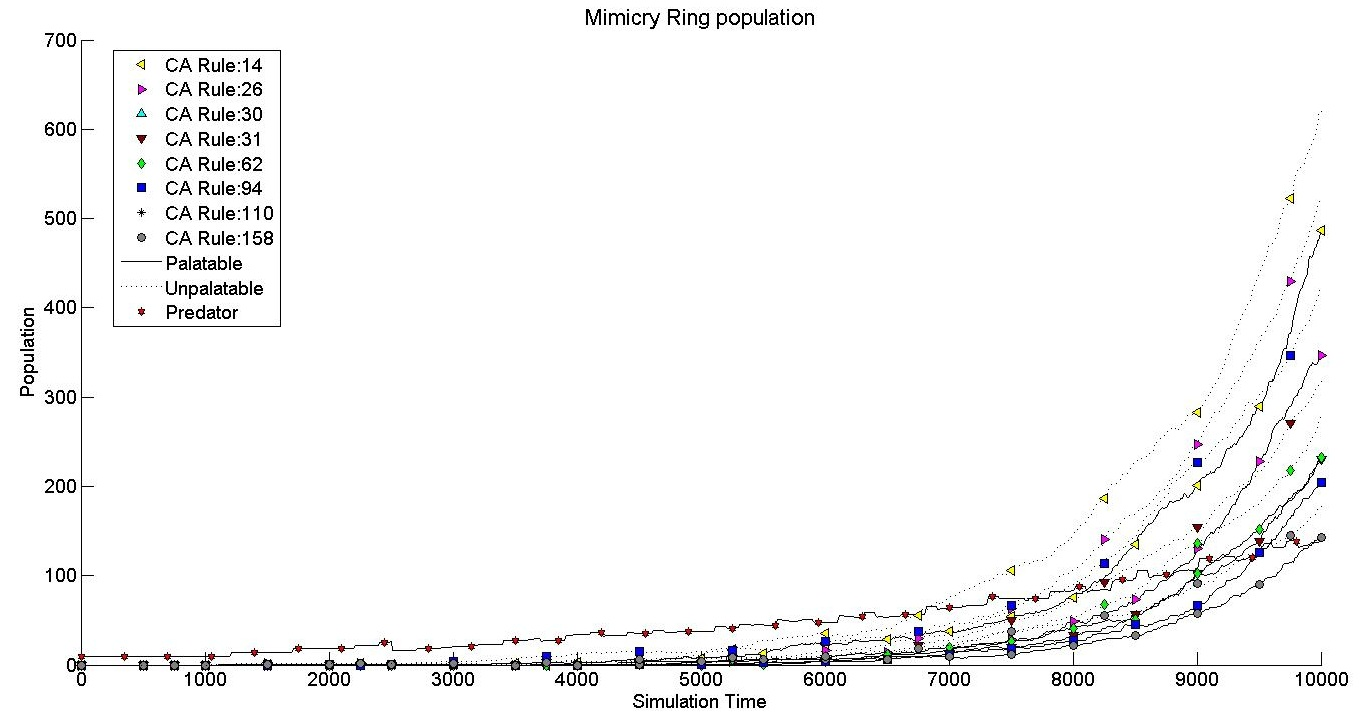
\includegraphics[scale=0.25]{../tex/images/simTime10k-2Prey-generated-prey}
		\caption{Population distribution of generated mimicry rings (2 prey species)}
		\label{fig:plot-2-prey-generated-prey}
	\end{figure}
}

%-----------------------------
%----- Four Prey Species ------
%-----------------------------
\frame
{
	\frametitle{Four Prey Species}
	\framesubtitle{Initial Configuration}

	\begin{table}
	\centering
	\begin{tiny}
	\begin{spacing}{1.5}
	\begin{tabular}{|l|l|c|c|l|c|}
	  \hline
	   														&\multicolumn{3}{c|}{Prey configuration} 																	
	   														& \multicolumn{2}{c|}{Predator configuration} \\ \hline
	  \multirow{4}{*}{Population} & Rule110 (Unpalatable) & \parbox[c]{2.1em}{
\includegraphics[scale=0.30]{../tex/images/CARule110}} 
	  																										& 50 & \multicolumn{2}{c|}{\multirow{4}{*}{10}} \\ \cline{2-4}
	  					 									& Rule30 (Palatable)& \parbox[c]{2.1em}{
\includegraphics[scale=0.30]{../tex/images/CARule30}}
	  					 																					& 50 & \multicolumn{2}{c|}{}\\ \cline{2-4}
	  					 									& Rule55 (Unpalatable)& \parbox[c]{2.1em}{
\includegraphics[scale=0.30]{../tex/images/CARule55}}
	  					 																					& 50 & \multicolumn{2}{c|}{}\\ \cline{2-4}
	  					 									& Rule190 (Palatable)& \parbox[c]{2.1em}{
\includegraphics[scale=0.30]{../tex/images/CARule190}}
	  					 																					& 50 & \multicolumn{2}{c|}{}\\ \hline
	  \multirow{2}{*}{Reproduction} & Age Limit & \multicolumn{2}{c|}{100}  & \multicolumn{2}{c|}{500} \\ \cline{2-6}
	  						 									& Interval  & \multicolumn{2}{c|}{1000} & \multicolumn{2}{c|}{\textbf{1400\(\uparrow\)}} \\ \hline
	  \multirow{2}{*}{Mutation Rate} & Pattern   & \multicolumn{2}{c|}{0.05} & \multicolumn{2}{c|}{\multirow{2}{*}{0.3}} \\ \cline{2-4}
	  						 									 & Genome    & \multicolumn{2}{c|}{0.5}  & \multicolumn{2}{c|}{} \\ \hline
	  Demise Age	 									 & \multicolumn{3}{c|}{2000}							& \multicolumn{2}{c|}{2500} \\ \hline
	  Minimum Attack Age						 & \multicolumn{3}{c|}{} 						    & \multicolumn{2}{c|}{500} \\ \hline
	  \multirow{2}{*}{Memory Configuration} & \multicolumn{3}{c|}{} 					& Minimum & \textbf{4\(\uparrow\)} \\ \cline{5-6}
	   																			& \multicolumn{3}{c|}{} 					& Maximum & 10 \\ \hline  
	\end{tabular}
	\end{spacing}
	\end{tiny}
	\caption{Agent configuration of 4 prey species}
	\label{tab:config-table-4-prey}
	\end{table}
}

\frame
{
	\frametitle{Four Prey Species}
	\framesubtitle{Population vs. Time (10k)}

	\begin{figure}
		\centering
		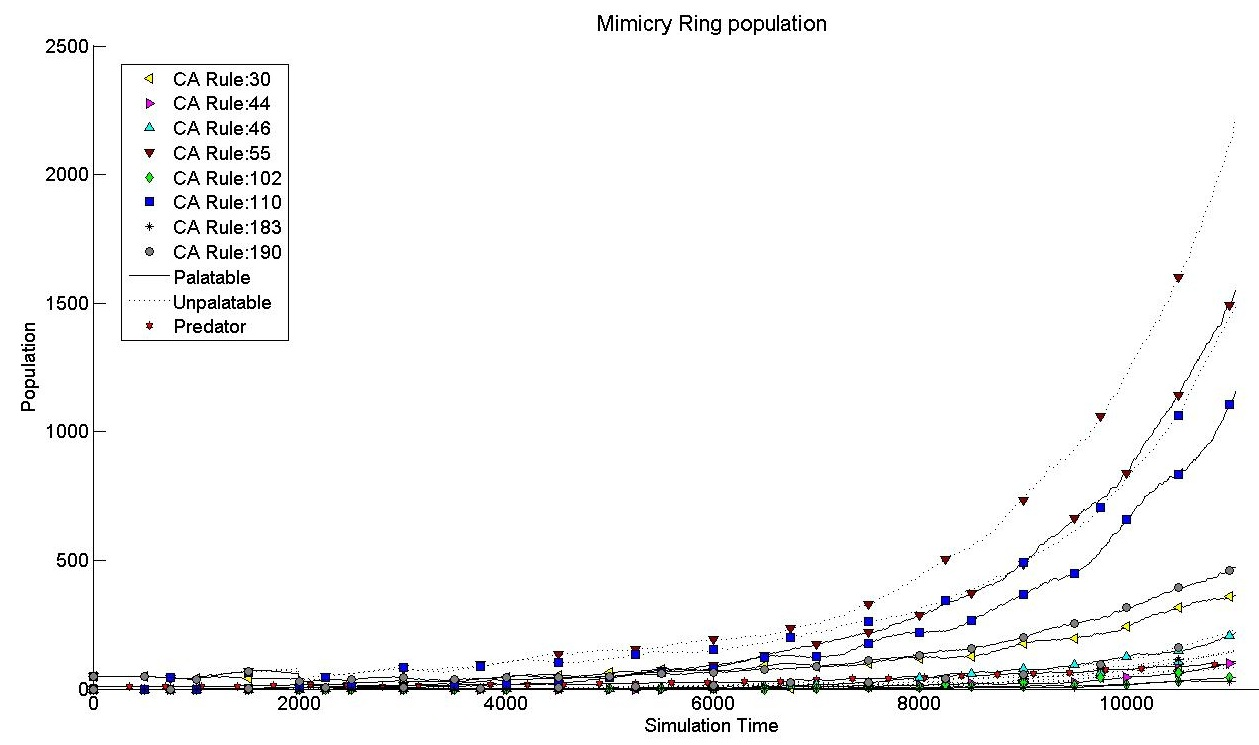
\includegraphics[scale=0.25]{../tex/images/simTime10k-4Prey}
		\caption{Population distribution of mimicry rings, initialized with 4 prey species.}
		\label{fig:plot-4-prey}
	\end{figure}
}

\frame
{
	\frametitle{Four Prey Species}
	\framesubtitle{Number of Mimicry Rings}

	\begin{figure}
		\centering
		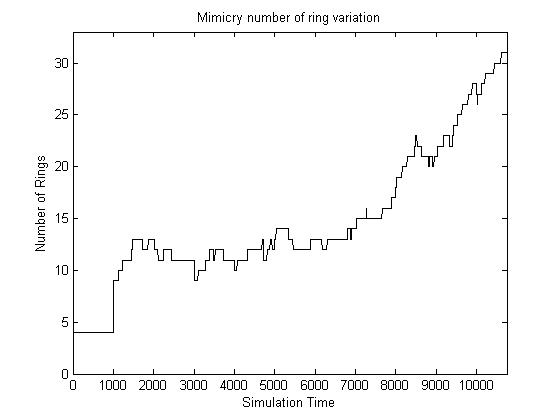
\includegraphics[scale=0.30]{../tex/images/ringSize10k-4Prey}
		\caption{Number of mimicry rings, initialized with 4 prey species.}
		\label{fig:ringSize10k-4Prey}
	\end{figure}
}

\frame
{
	\frametitle{Four Prey Species}
	\framesubtitle{Simulation Time: 11k}

	\begin{figure}[H]
		\centering
		\label{fig:screenshot-simTime11K-4Prey}
		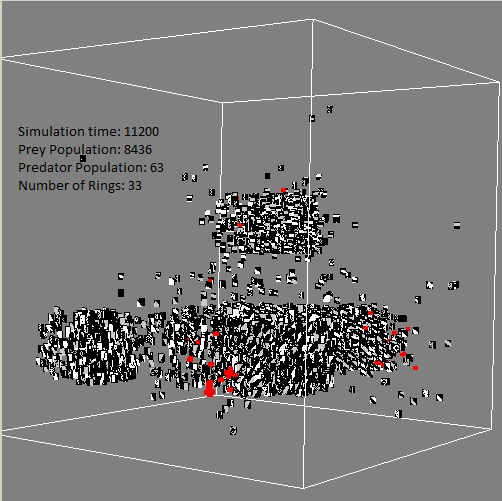
\includegraphics[scale=0.4]{../tex/images/simTime11K-4Prey}
		\caption{Graphical representation of the model (simulation time: 11200)}
	\end{figure}
}

%-----------------------------
%----- Four Prey Species ------
%-----------------------------
\frame
{
	\frametitle{Four Prey Species}
	\framesubtitle{Increased Population}

	\begin{table}[H]
	\centering
	\begin{tiny}
	\begin{spacing}{1.5}	
	\begin{tabular}{|l|l|c|c|l|c|}
	  \hline
	   														&\multicolumn{3}{c|}{Prey configuration} 																	
	   														& \multicolumn{2}{c|}{Predator configuration} \\ \hline
	  \multirow{4}{*}{Population} & Rule110 (Palatable) & \parbox[c]{2.1em}{
\includegraphics[scale=0.30]{../tex/images/CARule110}} & \textbf{150 \(\uparrow\)} & \multicolumn{2}{c|}{\multirow{4}{*}{\textbf{20 \(\uparrow\)}}} \\ \cline{2-4}
	  					 									& Rule30 (Palatable)& \parbox[c]{2.1em}{
\includegraphics[scale=0.30]{../tex/images/CARule30}}  	 & \textbf{150 \(\uparrow\)} & \multicolumn{2}{c|}{}\\ \cline{2-4}
	  					 									& Rule55 (Unpalatable)& \parbox[c]{2.1em}{
\includegraphics[scale=0.30]{../tex/images/CARule55}}  & \textbf{150 \(\uparrow\)} & \multicolumn{2}{c|}{}\\ \cline{2-4}
	  					 									& Rule190 (Unpalatable)& \parbox[c]{2.1em}{
\includegraphics[scale=0.30]{../tex/images/CARule190}}& \textbf{150 \(\uparrow\)} & \multicolumn{2}{c|}{}\\ \hline
	  \multirow{2}{*}{Reproduction} & Age Limit & \multicolumn{2}{c|}{100}  & \multicolumn{2}{c|}{500} \\ \cline{2-6}
	  						 									& Interval  & \multicolumn{2}{c|}{1000} & \multicolumn{2}{c|}{\textbf{2500 \(\uparrow\)}} \\ \hline
	  \multirow{2}{*}{Mutation Rate} & Pattern   & \multicolumn{2}{c|}{0.05} & \multicolumn{2}{c|}{\multirow{2}{*}{0.3}} \\ \cline{2-4}
	  						 									 & Genome    & \multicolumn{2}{c|}{0.5}  & \multicolumn{2}{c|}{} \\ \hline
	  Demise Age	 									 & \multicolumn{3}{c|}{2000}							& \multicolumn{2}{c|}{\textbf{7000 \(\uparrow\)}} \\ \hline
	  Minimum Attack Age						 & \multicolumn{3}{c|}{} 						    & \multicolumn{2}{c|}{500} \\ \hline
	  \multirow{2}{*}{Memory Configuration} & \multicolumn{3}{c|}{} 					& Minimum & 4 \\ \cline{5-6}
	   																			& \multicolumn{3}{c|}{} 					& Maximum & 10 \\ \hline  
	\end{tabular}
	\end{spacing}	
	\end{tiny}
	\caption{Agent configuration of 4 prey species with increased population}
	\label{tab:config-table-4-more-prey}
	\end{table}

}

\frame
{
	\frametitle{Four Prey Species}
	\framesubtitle{Increased Population\\ Population vs. Time (10k)}

	\begin{figure}[H]
		\centering
		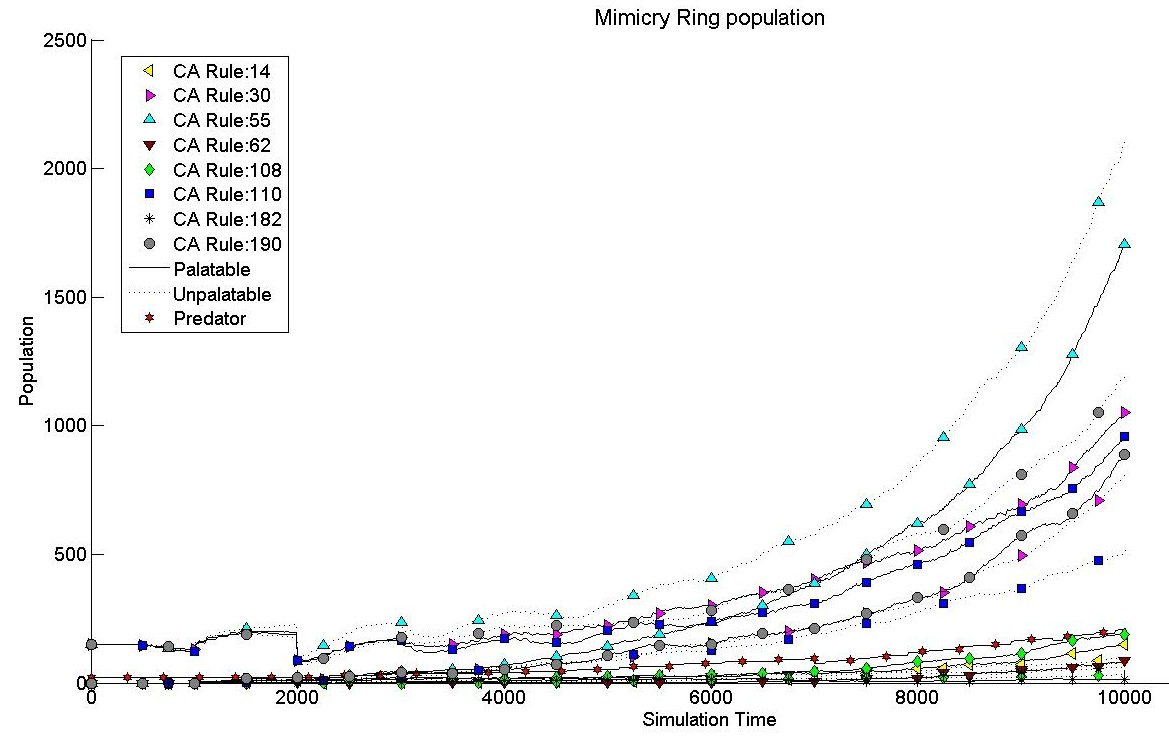
\includegraphics[scale=0.25]{../tex/images/simTime10K-4MorePrey}
		\caption{Population distribution of mimicry rings (4 prey species, increased population)}
		\label{fig:plot-4-more-prey}
	\end{figure}	
}

\frame
{
	\frametitle{Four Prey Species}
	\framesubtitle{Increased Population\\ Number of Mimicry Rings}
	
	\begin{figure}[H]
		\centering
		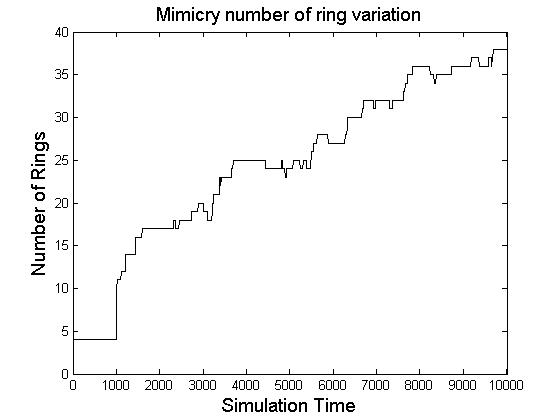
\includegraphics[scale=0.30]{../tex/images/ringSize10k-4MorePrey}
		\caption{Number of mimicry rings (4 prey species, increased population)}
	\end{figure}	
}

%-----------------------------
%----- Six Prey Species ------
%-----------------------------
\frame
{
	\frametitle{Six Prey Species}
	\framesubtitle{Initial Configuration}
	
	\begin{table}
	\centering
	\begin{tiny}
	\begin{spacing}{1.5}
	\begin{tabular}{|l|l|c|c|l|c|}
	  \hline
	   														&\multicolumn{3}{c|}{Prey configuration} 																	
	   														& \multicolumn{2}{c|}{Predator configuration} \\ \hline
	  \multirow{6}{*}{Population} & Rule110 (Palatable) & \parbox[c]{2.1em}{
\includegraphics[scale=0.30]{../tex/images/CARule110}} 
	  																									& 150 & \multicolumn{2}{c|}{\multirow{6}{*}{\textbf{30\(\uparrow\)}}} \\ \cline{2-4}
	  					 									& Rule30  (Unpalatable)& \parbox[c]{2.1em}{
\includegraphics[scale=0.30]{../tex/images/CARule30}}  
	  					 																				& 150 & \multicolumn{2}{c|}{}\\ \cline{2-4}
	  					 									& Rule55  (Palatable)& \parbox[c]{2.1em}{
\includegraphics[scale=0.30]{../tex/images/CARule55}}    
	  					 																				& 150 & \multicolumn{2}{c|}{}\\ \cline{2-4}
	  					 									& Rule190 (Unpalatable)& \parbox[c]{2.1em}{
\includegraphics[scale=0.30]{../tex/images/CARule190}} 
	  					 																				& 150 & \multicolumn{2}{c|}{}\\ \cline{2-4}
	  					 									& Rule57  (Palatable)& \parbox[c]{2.1em}{
\includegraphics[scale=0.30]{../tex/images/CARule57}}    
	  					 																				& 150 & \multicolumn{2}{c|}{}\\ \cline{2-4}
	  					 									& Rule105 (Unpalatable)& \parbox[c]{2.1em}{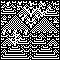
\includegraphics[scale=0.30]{../tex/images/CARule105}}& 150 & \multicolumn{2}{c|}{}\\ \hline
	  \multirow{2}{*}{Reproduction} & Age Limit & \multicolumn{2}{c|}{100}  & \multicolumn{2}{c|}{500} \\ \cline{2-6}
	  						 									& Interval  & \multicolumn{2}{c|}{1000} & \multicolumn{2}{c|}{2000} \\ \hline
	  \multirow{2}{*}{Mutation Rate} & Pattern   & \multicolumn{2}{c|}{0.05} & \multicolumn{2}{c|}{\multirow{2}{*}{0.3}} \\ \cline{2-4}
	  						 									 & Genome    & \multicolumn{2}{c|}{0.5}  & \multicolumn{2}{c|}{} \\ \hline
	  Demise Age	 									 & \multicolumn{3}{c|}{2000}							& \multicolumn{2}{c|}{7000} \\ \hline
	  Minimum Attack Age						 & \multicolumn{3}{c|}{} 						    & \multicolumn{2}{c|}{500} \\ \hline
	  \multirow{2}{*}{Memory Configuration} & \multicolumn{3}{c|}{} 					& Minimum & \textbf{6 \(\uparrow\)} \\ \cline{5-6}
	   																			& \multicolumn{3}{c|}{} 					& Maximum & 10 \\ \hline  
	\end{tabular}
	\end{spacing}
	\end{tiny}
	\caption{Agent configuration of 6 prey species.}
	\label{tab:config-table-6-prey}
	\end{table}
	
}

\frame
{
	\frametitle{Six Prey Species}
	\framesubtitle{Population vs. Time (10k)}

	\begin{figure}
		\centering
		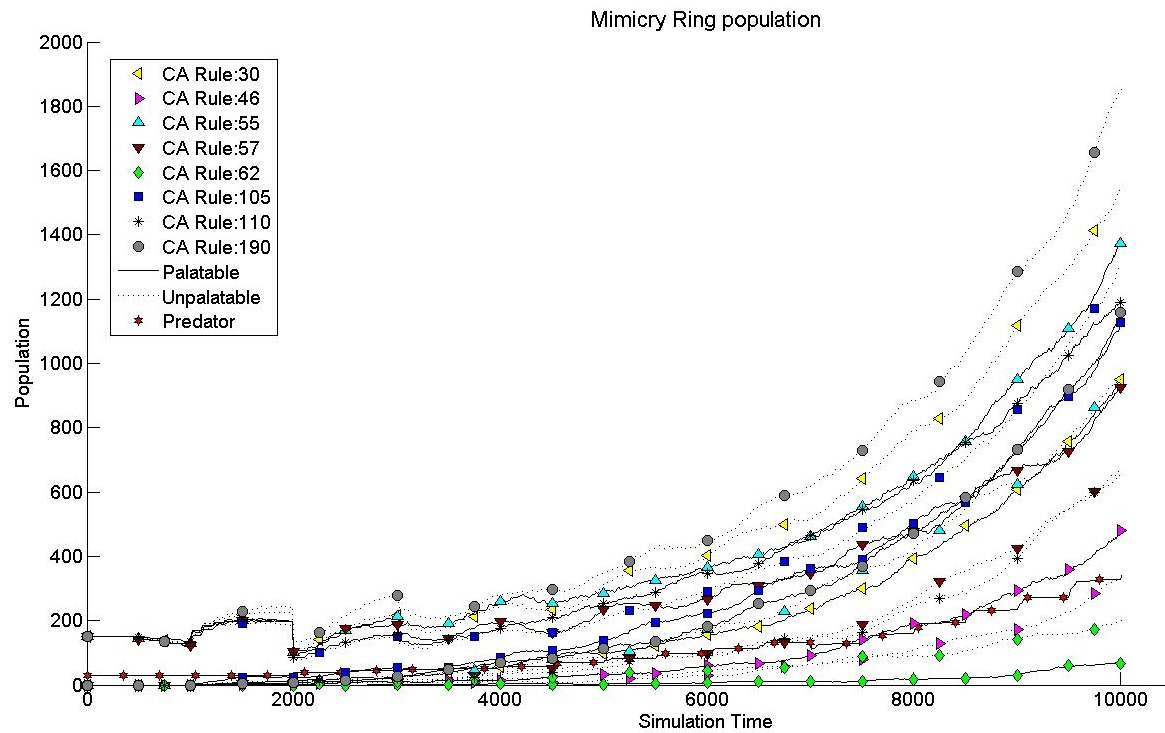
\includegraphics[scale=0.25]{../tex/images/simTime10k-6Prey}
		\caption{Population distribution of mimicry rings (6 prey species)}
		\label{fig:plot-6-prey}
	\end{figure}
}

\frame
{
	\frametitle{Six Prey Species}
	\framesubtitle{Number of Mimicry Rings}

	\begin{figure}[H]
		\centering
		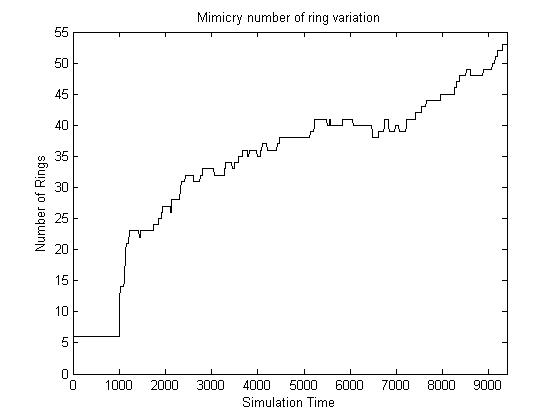
\includegraphics[scale=0.30]{../tex/images/ringSize10k-6Prey}
		\caption{Number of mimicry rings (6 prey species)}
		\label{fig:ringSize10k-6-Prey}
	\end{figure}	
}

%-----------------------------
%----- Unpalatable Species ------
%-----------------------------
\frame
{
	\frametitle{Only Unpalatable Species}
	\framesubtitle{Initial Configuration}

	\begin{table}[H]
	\centering
	\begin{tiny}
	\begin{spacing}{1.5}
	\begin{tabular}{|l|l|c|c|l|c|}
	  \hline
	   														&\multicolumn{3}{c|}{Prey configuration} 																	
	   														& \multicolumn{2}{c|}{Predator configuration} \\ \hline
	  \multirow{4}{*}{Population} & Rule110 (Unpalatable) & \parbox[c]{2.1em}{
\includegraphics[scale=0.30]{../tex/images/CARule110}} 
	  																									& 150 & \multicolumn{2}{c|}{\multirow{4}{*}{\textbf{20 \(\downarrow\)}}} \\ \cline{2-4}
	  					 									& Rule30  (Unpalatable)& \parbox[c]{2.1em}{
\includegraphics[scale=0.30]{../tex/images/CARule30}}  
	  					 																				& 150 & \multicolumn{2}{c|}{}\\ \cline{2-4}
	  					 									& Rule55  (Unpalatable)& \parbox[c]{2.1em}{
\includegraphics[scale=0.30]{../tex/images/CARule55}}    
	  					 																				& 150 & \multicolumn{2}{c|}{}\\ \cline{2-4}
	  					 									& Rule190 (Unpalatable)& \parbox[c]{2.1em}{
\includegraphics[scale=0.30]{../tex/images/CARule190}}& 150 & \multicolumn{2}{c|}{}\\ \hline
	  \multirow{2}{*}{Reproduction} & Age Limit & \multicolumn{2}{c|}{100}  & \multicolumn{2}{c|}{500} \\ \cline{2-6}
	  						 									& Interval  & \multicolumn{2}{c|}{1000} & \multicolumn{2}{c|}{2000} \\ \hline
	  \multirow{2}{*}{Mutation Rate} & Pattern   & \multicolumn{2}{c|}{0.05} & \multicolumn{2}{c|}{\multirow{2}{*}{0.3}} \\ \cline{2-4}
	  						 									 & Genome    & \multicolumn{2}{c|}{0.5}  & \multicolumn{2}{c|}{} \\ \hline
	  Demise Age	 									 & \multicolumn{3}{c|}{2000}							& \multicolumn{2}{c|}{\textbf{5000 \(\downarrow\)}} \\ \hline
	  Minimum Attack Age						 & \multicolumn{3}{c|}{} 						    & \multicolumn{2}{c|}{500} \\ \hline
	  \multirow{2}{*}{Memory Configuration} & \multicolumn{3}{c|}{} 					& Minimum & \textbf{4 \(\downarrow\)} \\ \cline{5-6}
	   																			& \multicolumn{3}{c|}{} 					& Maximum & 10 \\ \hline  
	\end{tabular}
	\end{spacing}
	\end{tiny}
	\caption{Agent configuration of 4 prey species all unpalatable.}
	\label{tab:config-table-4-prey-unpalatable}
	\end{table}	

}

\frame
{
	\frametitle{Only Unpalatable Species}
	\framesubtitle{Population vs. Time (10k)}

	\begin{figure}[H]
		\centering
		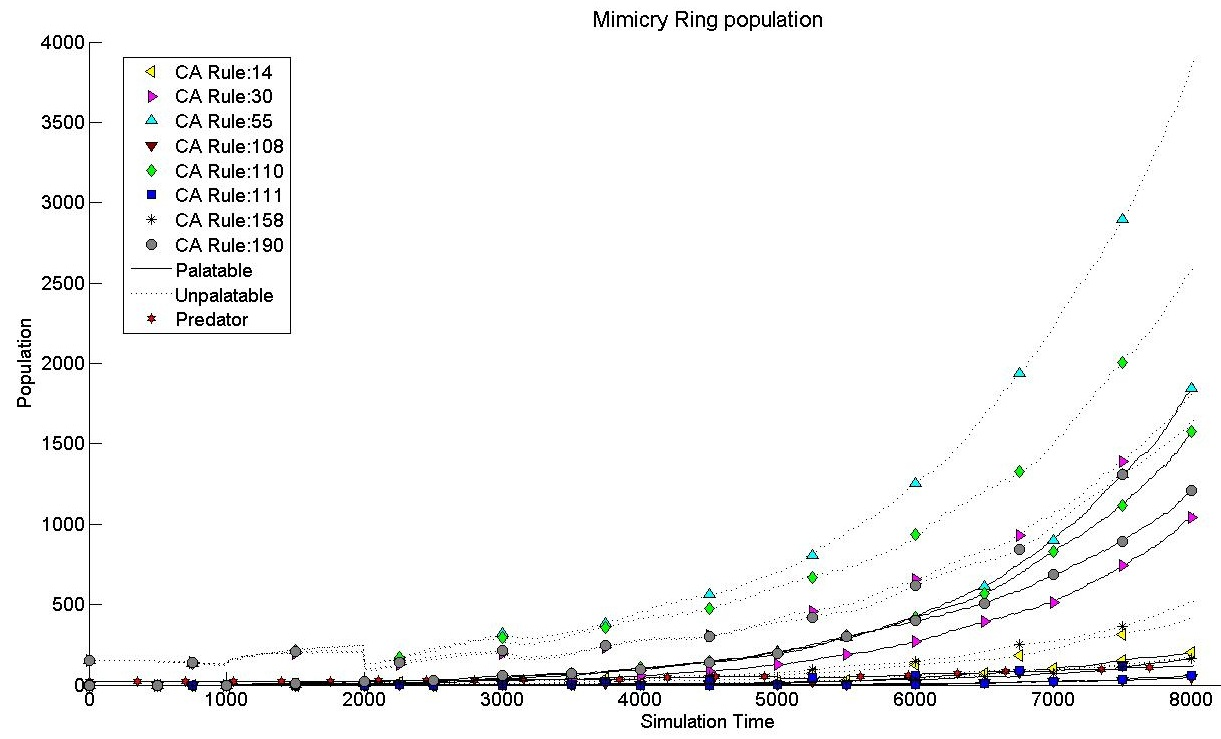
\includegraphics[scale=0.25]{../tex/images/simTime8k-4Prey-unp}
		\caption{Population distribution of mimicry rings(4 prey species all unpalatable)}
		\label{fig:plot-4-prey-unp}
	\end{figure}

}

\frame
{
	\frametitle{Only Unpalatable Species}
	\framesubtitle{Reduced Predator Memory\\ Population vs. Time (10k)}

	\begin{figure}[H]
		\centering
		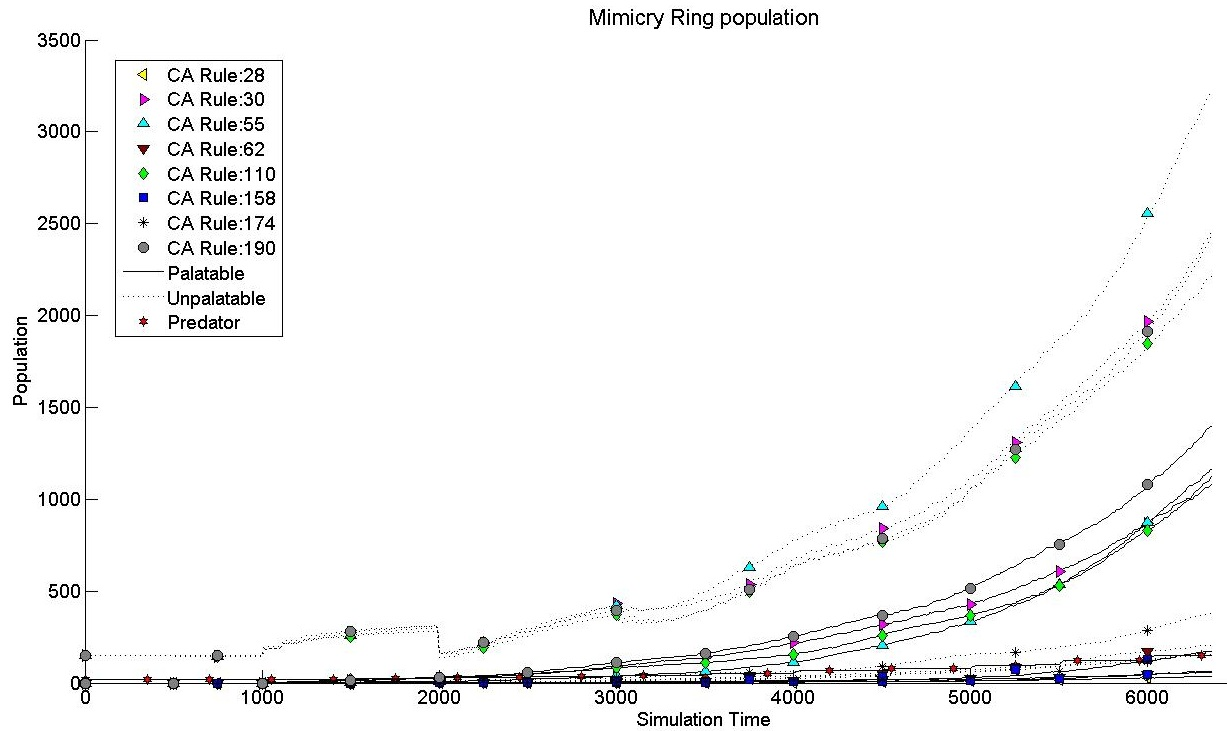
\includegraphics[scale=0.25]{../tex/images/simTime6k-4Prey-unp-1-mem}
		\caption{Population distribution of mimicry rings. 4 prey, all unpalatable but reduced predator memory}
		\label{fig:plot-4-prey-unp-1-mem}
	\end{figure}
}

%-----------------------------
%----- Palatable Species ------
%-----------------------------
\frame
{
	\frametitle{Only Palatable Species}
	\framesubtitle{Initial Configuration}

	\begin{table}[H]
	\centering
	\begin{spacing}{1.5}
	\begin{tiny}
	\begin{tabular}{|l|l|c|c|l|c|}
	  \hline
	   														&\multicolumn{3}{c|}{Prey configuration} 																	
	   														& \multicolumn{2}{c|}{Predator configuration} \\ \hline
	  \multirow{4}{*}{Population} & Rule110 (Palatable) & \parbox[c]{2.1em}{
\includegraphics[scale=0.30]{../tex/images/CARule110}} 
	  																									& 150 & \multicolumn{2}{c|}{\multirow{4}{*}{20}} \\ \cline{2-4}
	  					 									& Rule30  (Palatable)& \parbox[c]{2.1em}{
\includegraphics[scale=0.30]{../tex/images/CARule30}}  
	  					 																				& 150 & \multicolumn{2}{c|}{}\\ \cline{2-4}
	  					 									& Rule55  (Palatable)& \parbox[c]{2.1em}{
\includegraphics[scale=0.30]{../tex/images/CARule55}}    
	  					 																				& 150 & \multicolumn{2}{c|}{}\\ \cline{2-4}
	  					 									& Rule190 (Palatable)& \parbox[c]{2.1em}{
\includegraphics[scale=0.30]{../tex/images/CARule190}}& 150 & \multicolumn{2}{c|}{}\\ \hline
	  \multirow{2}{*}{Reproduction} & Age Limit & \multicolumn{2}{c|}{100}  & \multicolumn{2}{c|}{500} \\ \cline{2-6}
	  						 									& Interval  & \multicolumn{2}{c|}{1000} & \multicolumn{2}{c|}{2000} \\ \hline
	  \multirow{2}{*}{Mutation Rate} & Pattern   & \multicolumn{2}{c|}{0.05} & \multicolumn{2}{c|}{\multirow{2}{*}{0.3}} \\ \cline{2-4}
	  						 									 & Genome    & \multicolumn{2}{c|}{0.5}  & \multicolumn{2}{c|}{} \\ \hline
	  Demise Age	 									 & \multicolumn{3}{c|}{2000}							& \multicolumn{2}{c|}{5000} \\ \hline
	  Minimum Attack Age						 & \multicolumn{3}{c|}{} 						    & \multicolumn{2}{c|}{500} \\ \hline
	  \multirow{2}{*}{Memory Configuration} & \multicolumn{3}{c|}{} 					& Minimum & 4 \\ \cline{5-6}
	   																			& \multicolumn{3}{c|}{} 					& Maximum & 10 \\ \hline  
	\end{tabular}
	\end{tiny}
	\end{spacing}
	\caption{Agent configuration of 4 prey species all palatable.}
	\label{tab:config-table-4-prey-palatable}
	\end{table}

}

\frame
{
	\frametitle{Only Palatable Species}
	\framesubtitle{Population vs. Time (7k)}

\begin{figure}[H]
	\centering
	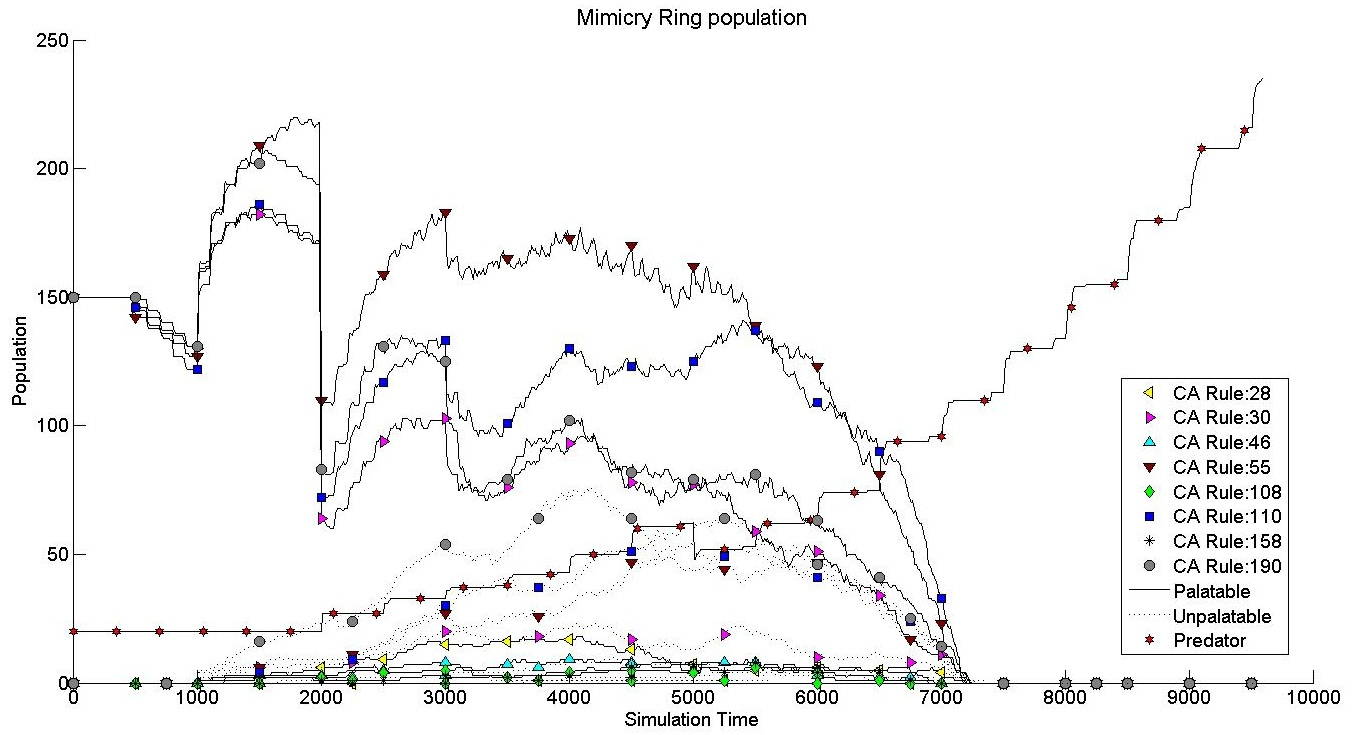
\includegraphics[scale=0.25]{../tex/images/simTime10k-4Prey-p}
	\caption{Population distribution of mimicry rings (4 prey species all palatable)}
	\label{fig:plot-4-prey-p}
\end{figure}
}


\frame
{
	\frametitle{Only Palatable Species}
	\framesubtitle{Number of Mimicry Rings}

	\begin{figure}[H]
		\centering
		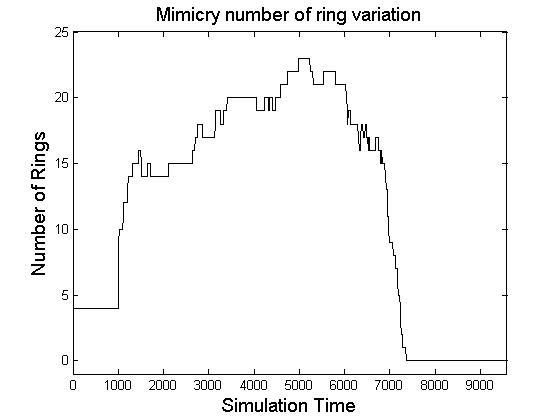
\includegraphics[scale=0.3]{../tex/images/ringSize10k-4Prey-p}
		\caption{Number of mimicry rings (4 prey species all palatable)}
		\label{fig:ringSize8k-4-Prey-p}
	\end{figure}
}

%-----------------------------
%----- Single Unpalatable ----
%-----------------------------
\frame
{
	\frametitle{Single Unpalatable Species}
	\framesubtitle{Initial Configuration}

	\begin{table}[H]
	\centering
	\begin{tiny}
	\begin{spacing}{1.5}
	\begin{tabular}{|l|l|c|c|l|c|}
	  \hline
	   														&\multicolumn{3}{c|}{Prey configuration} 																	
	   														& \multicolumn{2}{c|}{Predator configuration} \\ \hline
	  Population 									& Rule30 (Unpalatable) & \parbox[c]{2.1em}{
\includegraphics[scale=0.30]{../tex/images/CARule30}} 
	  																									& 216 & \multicolumn{2}{c|}{\textbf{10 \(\downarrow\)}} \\ \hline
	  \multirow{2}{*}{Reproduction} & Age Limit & \multicolumn{2}{c|}{100}  & \multicolumn{2}{c|}{500} \\ \cline{2-6}
	  						 									& Interval  & \multicolumn{2}{c|}{1000} & \multicolumn{2}{c|}{\textbf{2500 \(\uparrow\)}} \\ \hline
	  \multirow{2}{*}{Mutation Rate} & Pattern   & \multicolumn{2}{c|}{0.05} & \multicolumn{2}{c|}{\multirow{2}{*}{0.3}} \\ \cline{2-4}
	  						 									 & Genome    & \multicolumn{2}{c|}{0.5}  & \multicolumn{2}{c|}{} \\ \hline
	  Demise Age	 									 & \multicolumn{3}{c|}{2000}							& \multicolumn{2}{c|}{7000} \\ \hline
	  Minimum Attack Age						 & \multicolumn{3}{c|}{} 						    & \multicolumn{2}{c|}{500} \\ \hline
	  \multirow{2}{*}{Memory Configuration} & \multicolumn{3}{c|}{} 					& Minimum & \textbf{2 \(\downarrow\)} \\ \cline{5-6}
	   																			& \multicolumn{3}{c|}{} 					& Maximum & 10 \\ \hline  
	\end{tabular}
	\end{spacing}
	\end{tiny}
	\caption{Agent configuration of 1 prey species unpalatable.}
	\label{tab:config-table-1-prey-unpalatable}
	\end{table}

}

\frame
{
	\frametitle{Single Unpalatable Species}
	\framesubtitle{Population vs. Time (8k)}

	\begin{figure}[H]
		\centering
		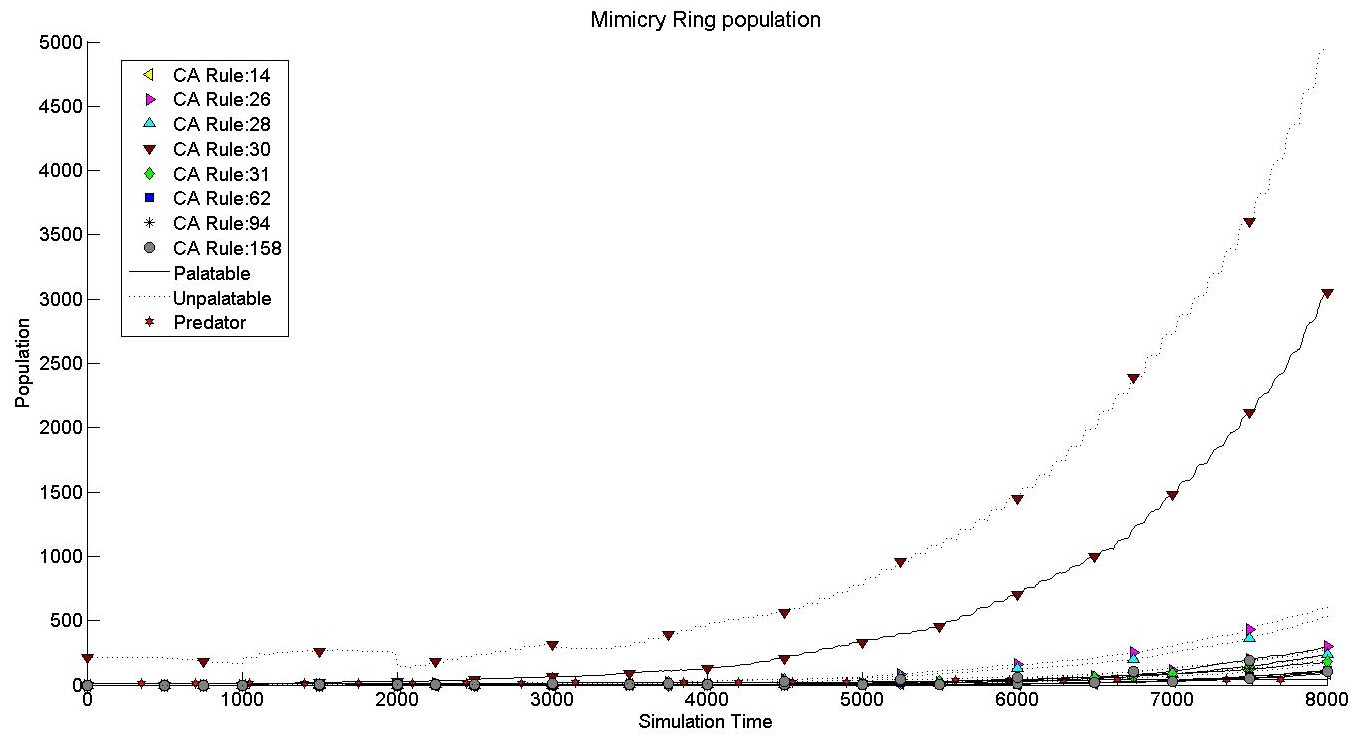
\includegraphics[scale=0.25]{../tex/images/simTime8k-1Prey-unp}
		\caption{Population distribution of mimicry rings (1 prey species unpalatable)}
		\label{fig:plot-1-prey-unp}
	\end{figure}

}

%-----------------------------
%----- Single Palatable ----
%-----------------------------
\frame
{
	\frametitle{Single Palatable Species}
	\framesubtitle{Initial Configuration}

	\begin{table}[H]
	\centering
	\begin{tiny}
	\begin{spacing}{1.5}
	\begin{tabular}{|l|l|c|c|l|c|}
	  \hline
	   														&\multicolumn{3}{c|}{Prey configuration} 																	
	   														& \multicolumn{2}{c|}{Predator configuration} \\ \hline
	  Population 									& Rule30 (Palatable) & \parbox[c]{2.1em}{
\includegraphics[scale=0.30]{../tex/images/CARule30}} 
	  																									& 216 & \multicolumn{2}{c|}{\textbf{8 \(\downarrow\)}} \\ \hline
	  \multirow{2}{*}{Reproduction} & Age Limit & \multicolumn{2}{c|}{100}  & \multicolumn{2}{c|}{500} \\ \cline{2-6}
	  						 									& Interval  & \multicolumn{2}{c|}{1000} & \multicolumn{2}{c|}{2500} \\ \hline
	  \multirow{2}{*}{Mutation Rate} & Pattern   & \multicolumn{2}{c|}{0.05} & \multicolumn{2}{c|}{\multirow{2}{*}{0.3}} \\ \cline{2-4}
	  						 									 & Genome    & \multicolumn{2}{c|}{0.5}  & \multicolumn{2}{c|}{} \\ \hline
	  Demise Age	 									 & \multicolumn{3}{c|}{2000}							& \multicolumn{2}{c|}{7000} \\ \hline
	  Minimum Attack Age						 & \multicolumn{3}{c|}{} 						    & \multicolumn{2}{c|}{500} \\ \hline
	  \multirow{2}{*}{Memory Configuration} & \multicolumn{3}{c|}{} 					& Minimum & 2 \\ \cline{5-6}
	   																			& \multicolumn{3}{c|}{} 					& Maximum & 10 \\ \hline  
	\end{tabular}
	\end{spacing}
	\end{tiny}
	\caption{Agent configuration of 1 prey species palatable.}
	\label{tab:config-table-1-prey-palatable}
	\end{table}
	
}

\frame
{
	\frametitle{Single Palatable Species}
	\framesubtitle{Population vs. Time (10k)}

	\begin{figure}[H]
		\centering
		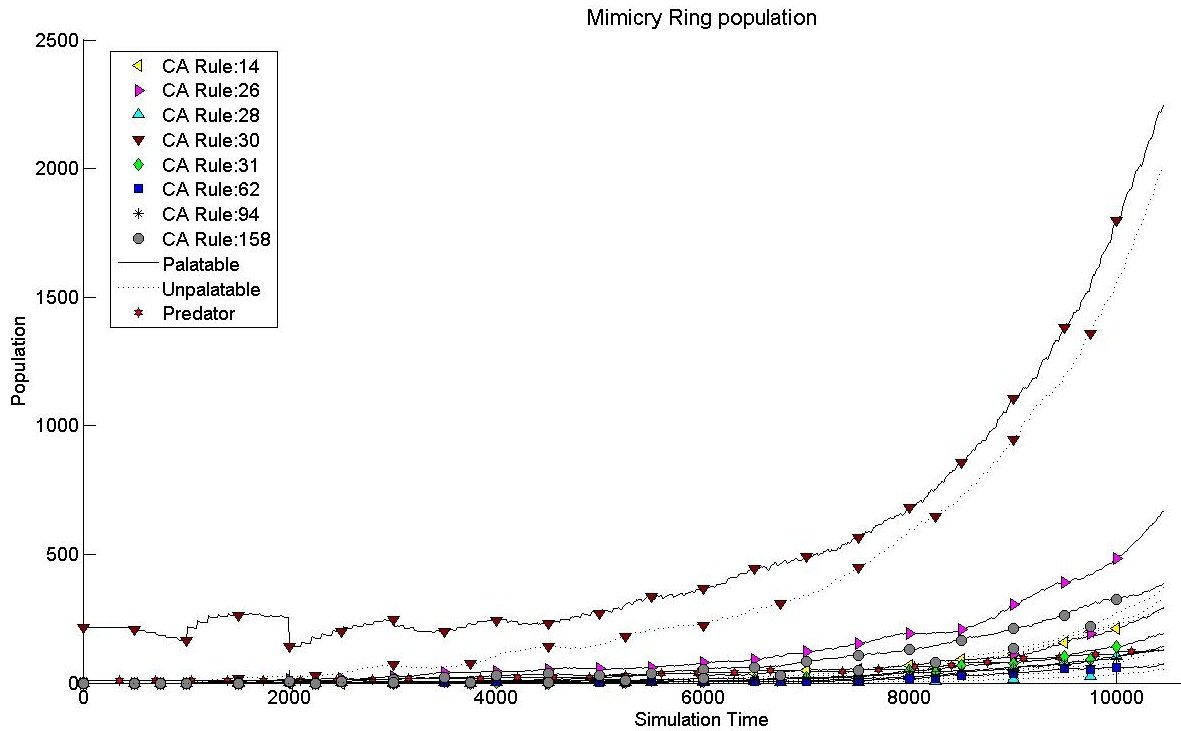
\includegraphics[scale=0.25]{../tex/images/simTime10k-1Prey-p}
		\caption{Population distribution of mimicry rings (1 prey species palatable)}
		\label{fig:plot-1-prey-p}
	\end{figure}
}

\subsection{Analysis}

\frame
{
	\frametitle{Analysis}
	\framesubtitle{Batesian Mimicry}

	\begin{itemize}
		\item Batesian Mimicry has taken effect, for all possible initial conditions.
			\begin{itemize}
				\item Every ring of unpalatable species there is a palatable ring.
			\end{itemize}
	\end{itemize}

	\begin{itemize}
		\item Start with palatable population, prey reaches extinction.\\
		\textbf{Reason:} No models to mimic for palatable species.
	\end{itemize}

	\begin{itemize}
		\item \textbf{Conclusion:} This model can simulate evolution of Batesian Mimicry.
	\end{itemize}

}

\frame
{
	\frametitle{Analysis}
	\framesubtitle{Mullerian Mimicry}

	\begin{quote}
		``Mullerian mimics converge into one large ring."
	\end{quote}
	
	\begin{itemize}
		\item Initialize simulation with 4 unpalatable species. No palatable ones.
		\item After 10k iteration all unpalatable species survive with dominance.
		\item \textbf{Reason:} Predator minimum memory configuration set to 4.
	\end{itemize}
	
	\begin{itemize}
		\item \textbf{New experiment:} reduce predator memory to 1.\\
		\item \textbf{Observation:} The phenomenon of single large ring do not occur. 
		\item \textbf{Conclusion:} Similar to Franks and Noble.\\
		Multiple Mullerian mimics do not converge into one large ring.
	\end{itemize}	
}

\frame
{
	\frametitle{Analysis}
	\framesubtitle{Conclusion}

	\begin{itemize}
		\item Successful simulation of evolution of mimicry.
		\item Accurate simulation of mimicry ring.\\
		Diverse new rings and shift in their population.
		\item Proof of the theory of Turner: evolution of mimicry with punctuated equilibrium.
	\end{itemize}
}